\subsection{Árboles de decisión}

Este modelo tiene la ventaja de ser muy rápido pero presenta el problema de que si se deja crecer mucho el árbol el clasificador puede sobre ajustar los datos de entrenamiento. Las primeras pruebas estuvieron orientadas estimar un rango de alturas en donde el clasificador tenga buena eficacia sin sobre ajustar. Para lograrlo calculamos la métrica  f0.5 de arboles de alturas de 1 a 30 para datos de entrenamiento y para cross validation con K=10. En la figura ~\ref{fig:arboles_f05_en_funcion_altura} puede ver un gráfico de los resultados.

\begin{figure}[H]
    \centering
        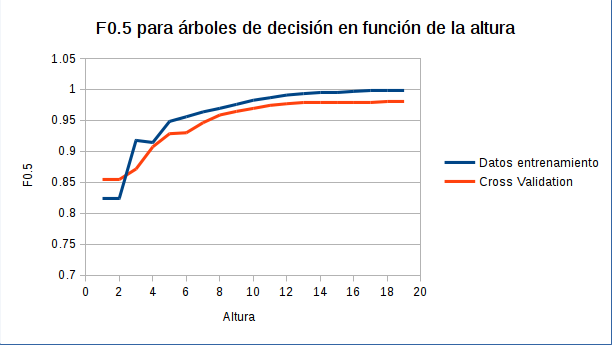
\includegraphics[width=\textwidth]{plots/arboles_f05_en_funcion_altura.png}
        \caption{f0.5 en función de la altura del árbol}
        \label{fig:arboles_f05_en_funcion_altura}
\end{figure}

	El resultado de cross validation es un estimador de la eficacia que vamos a obtener clasificando correos nuevos y a pesar de que por lo general no aproxime correctamente la eficacia nos permite predecir que estamos haciendo sobre ajuste de datos de entrenamiento cuando al aumentar la altura baja o se mantiene la eficacia. Como se puede ver en la figura ~\ref{fig:arboles_f05_en_funcion_altura} a partir de arboles de altura 9 el aumento en la eficacia al variar la altura especia a bajar hasta que se estanca llegando a arboles de altura 15.
    Luego para para este rango de alturas ejecutamos un grid search a fin de obtener los mejores hiper-parametros para el clasificador. 

 \begin{enumerate}
\item \textit{criterio de selección:} Se probaron criterios, gini y ganancia de información. No se observaron grandes diferencias en la eficacia del clasificador al variar el criterio. El mejor resultado se obtuvo con ganancia de información. 
\item \textit{Cantidad máxima de atributos considerados:} Este hiper-parámetro permite limitar la cantidad de atributos considerados al hacer un split.  Tiende a favorecer al aparición de arboles que no sean dominados por los atributos que provean mayor ganancia de información, dado que es posible que varios atributos más débiles trabajando en conjunto logren mejor eficacia.  En las pruebas realizadas se obtuvieron mejores resultados sin limitar la cantidad de atributos
\item \textit{Cantidad mínima de elementos en división:} Limita la división de nodos internos a lo que superen en cantidad de elementos la cantidad especificada. Los mejores resultados se obtuvieron con el valor mínimo de 2. Al aumentar el valor y al mismo tiempo limitar las cantidad de atributos limitados se puede observar una caída de eficacia en cross validation. 
\item \textit{Cantidad mínima de elementos en hojas:} Las hojas del árbol no pueden tener menos de la cantidad especificada. Los mejores resultados se obtuvieron con el valor mínimo de 2. Al igual que con el hiper-parámetro anterior, aumentar el valor y al mismo tiempo limitar las cantidad de atributos limitados se puede observar una caída de eficacia en cross validation.  

\subsection{Random Forest}


La idea de random forest es utlizar múltiples árboles de decisión para mejorar la eficacia del clasificador, reduciendo la alta varianza que se observa en la utilización de un único árbol. Esto es posible gracias al bajo costos que lleva entrenar y consultar a cada árbol. 
 La reducción en la varianza suele ser mas significativa cuando el bosque se arma con árboles que utilicen diferentes atributos. Para lograr esto los atributos utilizados en las divisiones de los nodo al construir el árbol se limitan a un subconjunto aleatorio de los atributos, reduciendo la probabilidad que lo atributos con mayor ganancia de información dominen todos los arboles. 
Utilizando los mismos parámetros que para el clasificador de un único árbol volvimos a hacer pruebas variando la cantidad de árboles del bosque y el tamaño del subconjunto de atributos a considerar. En la figura ~\ref{fig:forest_f05_en_funcion_de_cantidad_de_arboles} se muestran los resultados para bosques de diferentes tamaños considerando n, $\sqrt{n}$ y $\log(n)$ atributos, donde n es la cantidad total de atributos. Los bosques en loas cuales se consideran n atributos muestran mejores resultados, pero cuando consideran $\sqrt{n}$ atributos,  la varianza es inferior por lo que esperamos que la eficacia con datos nuevos sea más parecida a lo  que observamos con cross validation sobre datos de entrenamiento. 

\begin{figure}[H]
\begin{center}
\myss{0.45}{random_forest.pdf}{$f_{0.5}$ en funcíon de cantidad de árboles}{0.35}
\myss{0.45}{random_forest_var.pdf}{varianza enfuncíon de cantidad de árboles}{0.35}
\caption{Resultados grid search random forest}
\label{fig:forest_f05_en_funcion_de_cantidad_de_arboles}
\end{center}
\end{figure}

\subsection{K Vécinos Mas Cercanos}

Para este clasificador consideramos un enfoque parecido al de árbol de decisión, a fin de limitar las pruebas necesarias para conseguir los mejores hiperparámetros, primero realizamos tests variando la cantidad de vecinos,k, considerados y calculando f0.5 para cross validation de 10 folds. Obteniendo los resultados de la figura ~\ref{fig:knn_f05_en_funcion_vecinos} .
\begin{figure}[H]
    \centering
        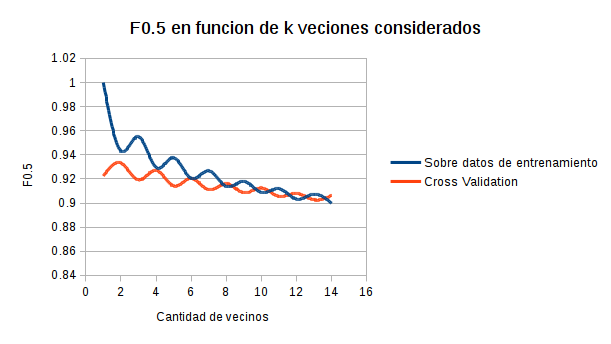
\includegraphics[width=\textwidth]{plots/knn_f05_en_funcion_vecinos.png}
        \caption{f0.5 en funcion de k vecinos considerados}
        \label{fig:knn_f05_en_funcion_vecinos}
\end{figure}
	A demás de la cantidad de vecinos este clasificador cuenta con los siguientes atributos:
 \begin{enumerate}
\item \textit{Peso:} Este parámetro ponderar el peso de cada uno de los vecinos según su distancia o puede tratarlos a todos uniformemente ignorando la distancia. En nuestro caso se obtuvieron mejores resultados considerando los vecinos uniformemente.  
\item \textit{Métrica de distancia:} Se probaron diferentes métricas de distancias, obteniendo los mejores resultados con la distancia manhattan en la cual la distancia entre dos puntos es la suma de las diferencias absolutas de sus coordenadas.
\end{enumerate}
	En el gráfico ~\ref{fig:knn_f05_en_funcion_vecinos} se observan los resultados del clasificador corriendo con los mejores atributos de \textit{Peso} y \textit{Métrica de Distancia} que encontramos para este problema.

\subsection{Naive Bayes}

Para este clasificador tuvimos que elegir primero la distribución que asumiriamos que iba a tener $ P(x_i | y) $, las opciones que consideramos fueron una distribución Gaussiana, Binomial y Multinomial. La distribución que mejores resultados obtuvo fue la Binomial lo cual tiene sentido debido a que modela bien la gran cantidad de atributos binarios, quizas si estos tuvieran mas de dos resultados posibles la distribución Multinomial o la Gaussiana habrian sido mejores opciónes.
Los hiperparametros que consideramos fueron $alpha$ y $fit\_prior$ , el primero suaviza la función de distribución de cada atributo y el segundo intenta ir mejorando la estimación de los atributos y las clases a priori, a medida que va analizando nuevas instancias.

\begin{figure}[H]
    \centering
        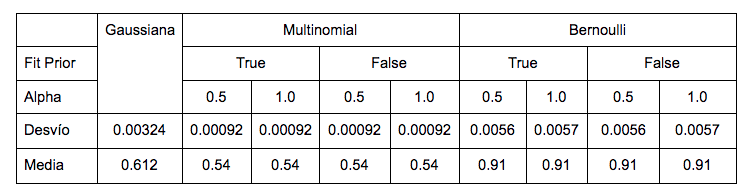
\includegraphics[width=\textwidth]{plots/tabla_nb.png}
        \caption{Media y Desvío Estandar de Clasificadores Naive Bayes luego de aplicar Cross Validation}
        \label{fig:nb_f05}
\end{figure}

\subsection{Support Vector Machine}

Debido a limitaciones de tiempo y computo solo pudimos probar SVM con los parametros dados por defecto en Sklearn \footnote{\url{http://scikit-learn.org/stable/modules/generated/sklearn.svm.SVC.html\#sklearn.svm.SVC}}, obtuvimos una performance del 83.5\% al realizar cross validation de 10 folds con el set de entrenamiento utilizando F0.5 como medida de score.

El clasificador con los parametros por defecto contiene como características principales un Kernel de Base Radial \footnote{\url{https://en.wikipedia.org/wiki/Radial_basis_function_kernel}} con parametro gamma = 1/numero\_de\_features y la heuristica llamada \textit{Shrinking} la cual permite realizar los computos del Kernel de forma mas rápida.

\end{enumerate}
